% !TeX root = ../index.tex
\documentclass[../index.tex]{subfiles}

\begin{document}
    \section{Wykład}
        Układ słoneczny zbudowany jest z \textbf{planet}, \textbf{planet karłowatych}, \textbf{księżyców} (naturalnych satelitów planet lub planet karłowatych), \textbf{planetoid} (inaczej asteroidy), \textbf{komet} i \textbf{meteoroidów}(drobne obiekty, do 10 m).\\
        Planety to obiekty okrążające gwiazdę, w których nie zachodzą reakcje syntezy jądrowej, o kulistym kształcie i dominujące w przestrzeni wokół swojej orbity. Planety karłowate różnią się od nich tym, że nie oczyściły sąsiedztwa swojej orbity z innych obiektów o porównywalnych rozmiarach. Planetoidy i komety, to obiekty o rozmiarach nie przekraczających kilkuset kilometrów, o stałej powierzchni i nieregularnym kształcie. Dodatkowo komety zawierają sporo lodu. \\
        Planety układu słonecznego to: \textbf{Merkury}, \textbf{Wenus}, \textbf{Ziemia}, \textbf{Mars}, \textbf{Jowisz}, \textbf{Saturn}, \textbf{Neptun} i \textbf{Uran}. Płaszczyzny orbit wszystkich planet zawierają się w kącie o rozwartości kilku stopni. \textbf{Pluton} uważany był za planetę, do 2006 roku, gdy odkryto w podobnej odległości od słońca innych obiektów o porównywalnych rozmiarach – \textbf{pas Kuipera}. Temperatura planet maleje wraz z odległością od Słońca (wyjątkiem jest Wenus, na której zachodzi efekt cieplarniany). Rzeczywista skala orbit planetarnych:
        \begin{center}
            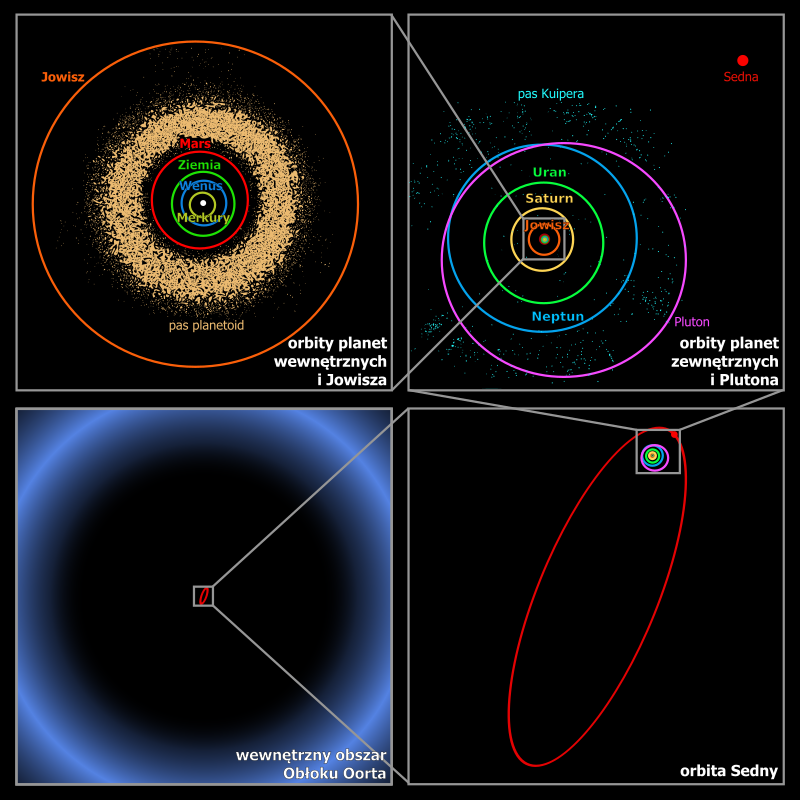
\includegraphics[width=12cm]{images/orbityPlanet}
        \end{center}
        Planety dzielą się na \textbf{planety skaliste} (Merkury, Wenus, Ziemia i Mars) i \textbf{gazowe olbrzymy}(Jowisz, Saturn, Uran i Neptun). Planety skaliste znajdują się bliżej Słońca, ich okresy obiegu są krótsze, a okresy obrotu dłuższe. Są także mniejsze i mniej masywne, ale za to bardziej gęste od gazowych olbrzymów. Gazowe olbrzymy mają dużo więcej satelitów i posiadają pierścienie. Każda grupa planet ma swój pas planetoid – jeden skalisty pomiędzy Marsem i Jowiszem oraz drugi zbudowany w dużym procencie z lodu pas Kuipera. Z tego drugie pochodzi większość komet. Kolizje albo jakiś inny rodzaj perturbacji powoduje, że taki obiekt trafią na orbitę, której peryhelium znajduje się w odległości kilku jednostek astronomicznych od Słońca. Lód zaczyna sublimować i wokół rozmarzającego obiektu powstaje gigantyczna głowa, którą rozwiewa wiatr słoneczny i ciśnienie promieniowania tworząc warkocz. Każde zbliżenie się komety do Słońca kosztuje ją część masy. Niektóre komety pochodzą z jeszcze odleglejszych peryferii Układu Słonecznego – \textbf{obłoku Oorta}. Sięga ona 100 000 jednostek astronomicznych, gdzie oddziaływanie grawitacyjne Słońca równoważone jest przez oddziaływanie innych gwiazd.\\
        Słońce oraz wszystkie pozostałe elementy Układu Słonecznego powstały z tego samego fragmentu obłoku molekularnego, który zaczął się zapadać pod własnym ciężarem 4.6 mld lat temu. Wraz z postępem kolapsu pojawiła się rotacja, która spowodowała w niektórych obszarach zatrzymanie się zapadania ku środkowi. W ten sposób wokół proto–Słońca uformował się \textbf{dysk protoplanetarny}. Stopniowo w dysku następowały procesy kondensacji cząsteczek gazu na ziarnach pyłu. Ze względu na różne wartości temperatury bliżej Słońca powstawały wyłącznie okruchy metali i skał, a w większej odległości równie lodu gazów takich jak \(H_2 O\), \(CO_2\), \(NH_3\), \(CH_4\) czy \(N_2\). W wyniku zderzeń okruchy sklejały się ze sobą tworząc coraz większe obiekty zwane \textbf{planetozymalami}, które w wyniku dalszych kolizji tworzyły zalążki planet.\\
        W kilka milionów lat uformowały się zalążki gazowych olbrzymów. Najwięcej materii było tuż za \textbf{granicą śniegu} (5-10 jednostek astronomicznych) i tam uformowały się Jowisz i Saturn. Od pewnego momentu ich grawitacja pozwoliła na bezpośrednia zbieranie materii z dysku. Uran i Neptun prawdopodobnie uformowały się bliżej Słońca niż są dziś i zostały wypchnięte przez Jowisz i Saturna (tam gdzie się dziś znajdują było zbyt mało materii do uformowania się planet).\\ 
        Proces formowania się planet skalistych trwał około kilkudziesięciu milionów lat. Materii w dysku o wysokiej temperaturze topnienie było niewiele, stąd małą łączna masa tych planet. Ponadto w pewnym momencie Słońce rozproszyło pozostałą część pyłu i gazu, co oznaczało, że dalszy wzrost planet wiązał się wyłącznie ze sklejania się planetozymali. W tym etapie najprawdopodobniej, w wyniku kolizji z inną protoplanetą, z Ziemi wyodrębnił się Księżyc.\\
        Proces wypychania Urana i Neptuna spowodował olbrzymie zamieszanie w licznej wówczas populacji planetozymali, które miały zbyt dużo miejsca, aby uformować jeszcze jedną planetę. Część z nich opuściła Układ Słoneczny, a inne zaczęły docierać bliżej Słońca inicjując \textbf{Wielkie Bombardowanie}. Nadal można obserwować jego skutki poprzez: kratery na powierzchni Merkurego i Księżyca, wsteczną rotację Wenus, całkowicie pochyloną względem płaszczyzny oś rotacji Urana (rotuje „na boku”) i wsteczny ruch obiegowy Trytona – największego księżyca Neptuna. W uformowaniu się planety pomiędzy Marsem a Jowiszem przeszkodziła grawitacja tego drugiego, który wypchnął większość planetozymali, a pozostałą reszta tworzy dziś pas planetoid.\\
        W 1992 r. Andrzej Wolszczan dowiódł istnienia planet wokół pewnego pulsara – planet poza Układem Słonecznym. Od tego czasu odkryto mnóstwo egzoplanet różnymi metodami: \textbf{chronometrażem pulsarowym}, \textbf{bezpośrednim obrazowaniem}, metodą \textbf{zmiany prędkości radialnej}, \textbf{metodą tranzytów} (obserwacja planety w trakcie przechodzenia na tle gwiazdy), metodą obserwacji \textbf{mikrosoczewkowania grawitacyjnego} oraz metodą obserwacji \textbf{przerw w dysku protoplanetarnym}.\\
        \textbf{Strefa życia} – zakres odległości pozwalających na obecność na planecie wody w stanie ciekłym, to parametr charakteryzujący gwiazdę. W kontekście poszukiwania życia pozaziemskiego szuka się egzoplanet mieszczących się w tej strefie.
\end{document}